\subsubsection{Effect of Pile-up on Dijet Balance}

The \pt{} balance of dijets events can be used to construct a correction factor or used to ascertain aspects of the JES uncertainty \cite{ref:JES}.
In this section it is used as a cross-check of JES uncertainty components from pile-up.
This is done by calculating the relative response for events with different levels of pile-up.

Two estimators of the amount of pile-up used are the number of primary vertices, $\mathrm{N_{PV}}$, and the mean number of interactions per bunch crossing, $\mu$.
Figure \ref{JetPerf:NPV_Mu} shows (a) the $\mathrm{N_{PV}}$ distribution and (b) the $\mu$ distributions.
$\mathrm{N_{PV}}$ and $\mu$ cuts are chosen to select events with different amount of pile-up.
For the $\mathrm{N_{PV}}$ cuts, three slices are chosen such that each has good statistics, but also has differences in the average $\mathrm{N_{PV}}$ per slice.
Three $\mathrm{N_{PV}}$ regions are defined to select different pile-up conditions, \Range{\mathrm{N_{PV}}}{0}{2}, \Range{\mathrm{N_{PV}}}{3}{6}, and  $\rm \mathrm{N_{PV}}\ge7$, with an average $\mathrm{N_{PV}}$ of 2.48, 4.48 and 7.71, respectively. 
For the $\mu$ cuts, two slices are chosen, one that includes the peak, and one that includes the tail, both of with have good statistics. 
Two $\mu$ regions are defined, \Range{\mu}{0}{7} and  $\mu > 7$, with an average $\mu$ of 5.33 and 9.94, respectively. 
Data points which have no cuts on $\mu$ or $\mathrm{N_{PV}}$ are also shown for comparative purposes.
These have an average $\mathrm{N_{PV}}$ and $\mu$ of 5.19 and 6.48, respectively.



%High NPV:  Ave NVP:  7.71314
%Med NPV:  Ave NVP:  4.48111
%Low NPV:  Ave NVP:  2.47613
%Standard: Average mu : 6.47532  Ave NVP:  5.18579


Figures \ref{JetPerf:PileupComp_j10}, \ref{JetPerf:PileupComp_j15} and \ref{JetPerf:PileupComp_j20}  show the relative response as a function of detector $\eta$ for jets with $22<\ptave{}<30$ GeV, $30<\ptave{}<40$ GeV and $55<\ptave{}<75$ GeV, respectively, for different $\mathrm{N_{PV}}$ ranges.
For the $22<\ptave{}<30$ GeV jets, the relative response in the forward bins is lower for jets in the low pile-up conditions than the jets using the full data.
The medium has a higher relative response in the bins outside the reference region.
The spread of the three different $\mathrm{N_{PV}}$ points is contained within $\approx 4\%$ and there is no systematic difference in spread as a function of $\eta{}$.
For the $30<\ptave{}<40$ GeV jets, the spread has decreased to within $\approx 2\%$. 
In the forward bins at negative $\eta$, the low pile-up and high pile-up have a higher and lower response than the average, respectively, however this is probably just fluctuations as there is no pathological effect.
For the  $55<\ptave{}<75$ GeV jets, the spread is within $\approx 1\%$, and there is no obvious trend in the differences between the different pile-up conditions.

The observation that the low \ptave{} jets are affected more, is not unexpected, as pile-up can be considered to add a fixed amount of additional energy per additional proton-proton interaction.
This additional energy will be a larger fraction of a low \pt{} jet than of a high \pt{} jet at the same rapidity, and so the net effect will be larger.
It might be expected that the jets in the lower pile-up conditions should have a lower relative response than jets in a higher pile-up condition, however the EM+JES calibration does an pile-up offset correction, which should account for this.


Figures \ref{JetPerf:MuComp_j10}, \ref{JetPerf:MuComp_j15} and \ref{JetPerf:MuComp_j20}  show the relative response as a function of detector $\eta$ for jets with $22<\ptave{}<30$ GeV, $30<\ptave{}<40$ GeV and $55<\ptave{}<75$ GeV respectively for different $\mu$ ranges.
For the $22<\ptave{}<30$ GeV jets, the spread  is $\approx 3\%$ for $-2.8\le\eta\le-2$ range, but for most bins it is within $ 1-2\%$.
In most of the bins the low pile-up sample has a responses slightly higher than the response from the high pile-up samples.
For the $30<\ptave{}<40$ GeV jets, the relative responses are closer to unity than for the lower \ptave{} jets.
The spread is consistent $2\%$ with approximately equal number of bins where the low pile-up sample is above the high pile-up sample, than the reverse.
For the $55<\ptave{}<75$ jets, the spread is $<1\%$ for all but one bin, and the relative response is close to one.  
As with the assessment of the pile-up using the $\mathrm{N_{PV}}$, the spread shows a general downwards trend for higher \ptave{}, though the jets with $30<\ptave{}<40$ GeV have a marginally higher spread than $22<\ptave{}<30$ GeV, but without the larger fluctuations,

The observed effects from $\mathrm{N_{PV}}$ and $\mu$ are $~3-4\%$ for low \ptave{} jets, and reduce to $~1\%$ for jets with $55<\ptave{}<75$.
These spreads of values for the relative response show agreement to the JES uncertainty due to pile-up using the method described in \cite{ref:Pileup} and combined to the JES uncertainty in \cite{ref:JES2011}.



\begin{figure}
\centering
        \begin{subfigure}[b]{0.5\textwidth}
                \centering
                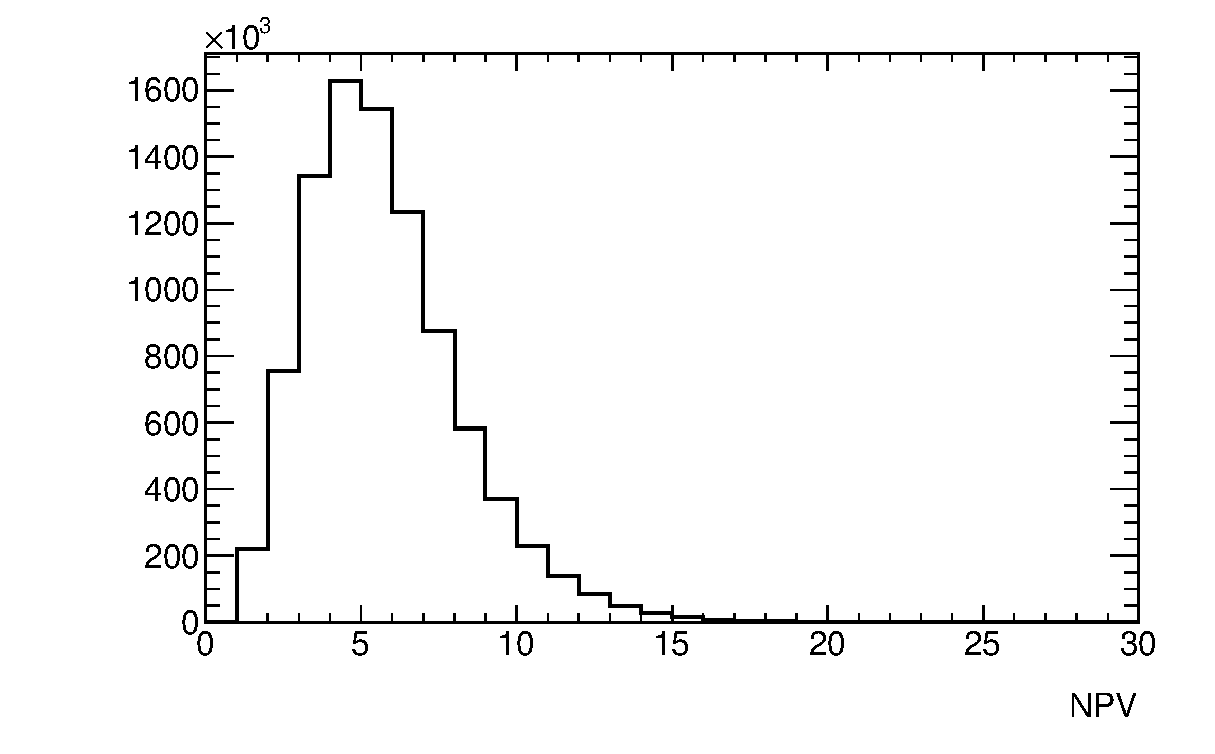
\includegraphics[width=\textwidth]{figures/JetPerformance/2011/NPVDist.eps}
        \end{subfigure}%
        \begin{subfigure}[b]{0.5\textwidth}
                \centering
                \includegraphics[width=\textwidth]{figures/JetPerformance/2011/MuDist.eps}
        \end{subfigure}%
\caption[Number of primary vertices and $\mu{}$ for 2011 data]{
(a) The $\mathrm{N_{PV}}$ distribution and (b) the $\mu$ distribution for 2011 data.
\label{JetPerf:NPV_Mu}}
\end{figure}



\begin{figure}
\centering
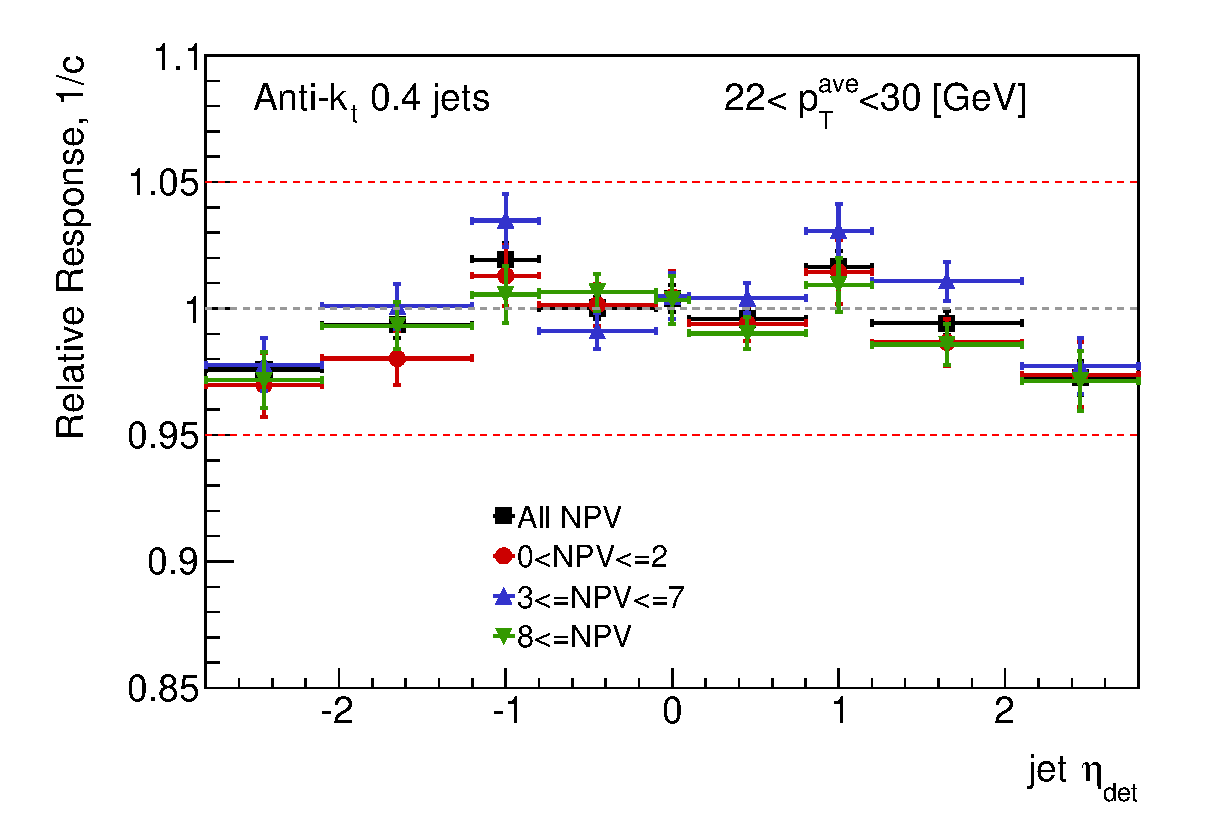
\includegraphics[width=0.9\textwidth]{figures/JetPerformance/2011/ResponseNPVj10Comp.eps}
\caption[Relative response as a function of $\eta$ for 3 different pile-up conditions, based on $\mathrm{N_{PV}}$, for jets with $22<\ptave{}<30$ GeV]{
Relative response as a function of detector $\eta$ for jets with $22<\ptave{}<30$ GeV.
Relative responses are shown for events with \Range{\mathrm{N_{PV}}}{0}{2}, \Range{\mathrm{N_{PV}}}{3}{6}, $\rm \mathrm{N_{PV}}\ge7$ and all $\mathrm{N_{PV}}$. 
\label{JetPerf:PileupComp_j10}}
\end{figure}



\begin{figure}
\centering
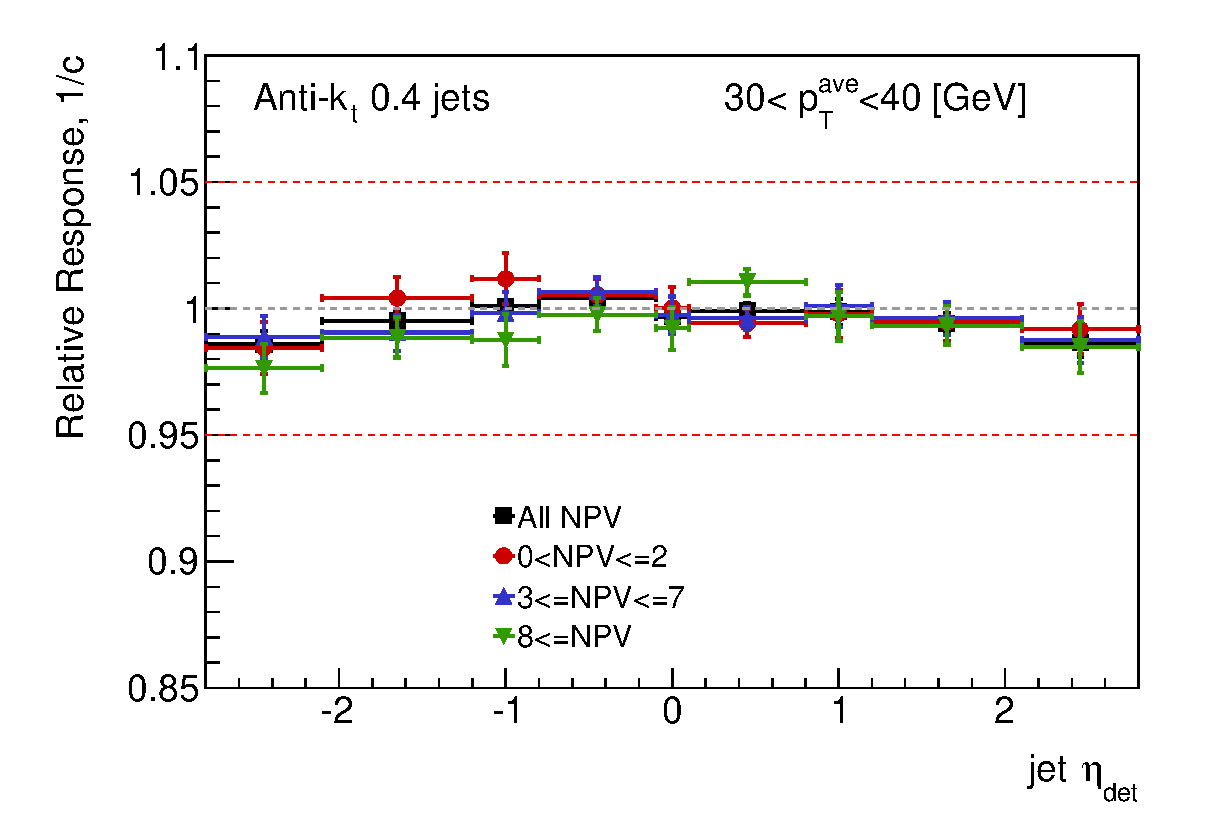
\includegraphics[width=0.9\textwidth]{figures/JetPerformance/2011/ResponseNPVj15Comp.eps}
\caption[Relative response as a function of $\eta$ for 3 different pile-up conditions, based on $\mathrm{N_{PV}}$, for jets with $30<\ptave{}<40$ GeV]{
Relative response as a function of detector $\eta$ for jets with $30<\ptave{}<40$ GeV.
Relative responses are shown for events with \Range{\mathrm{N_{PV}}}{0}{2}, \Range{\mathrm{N_{PV}}}{3}{6}, $\rm \mathrm{N_{PV}}\ge7$ and all $\mathrm{N_{PV}}$. 
\label{JetPerf:PileupComp_j15}}
\end{figure}

\begin{figure}
\centering
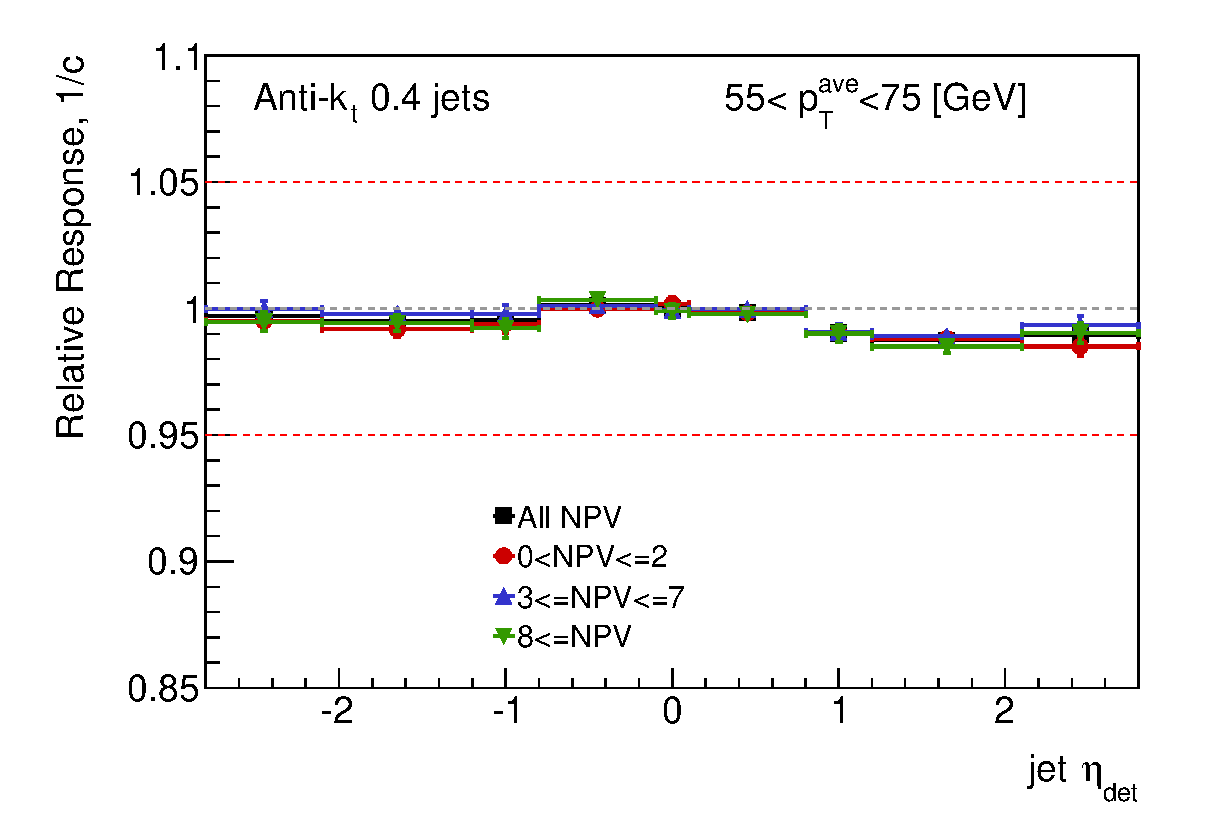
\includegraphics[width=0.9\textwidth]{figures/JetPerformance/2011/ResponseNPVj30Comp.eps}
\caption[Relative response as a function of $\eta$ for 3 different pile-up conditions, based on $\mathrm{N_{PV}}$, for jets with $55<\ptave{}<75$ GeV]{
Relative response as a function of detector $\eta$ for jets with $55<\ptave{}<75$ GeV.
Relative responses are shown for events with \Range{\mathrm{N_{PV}}}{0}{2}, \Range{\mathrm{N_{PV}}}{3}{6}, $\rm \mathrm{N_{PV}}\ge7$ and all $\mathrm{N_{PV}}$. 
\label{JetPerf:PileupComp_j20}}
\end{figure}

\begin{figure}
\centering
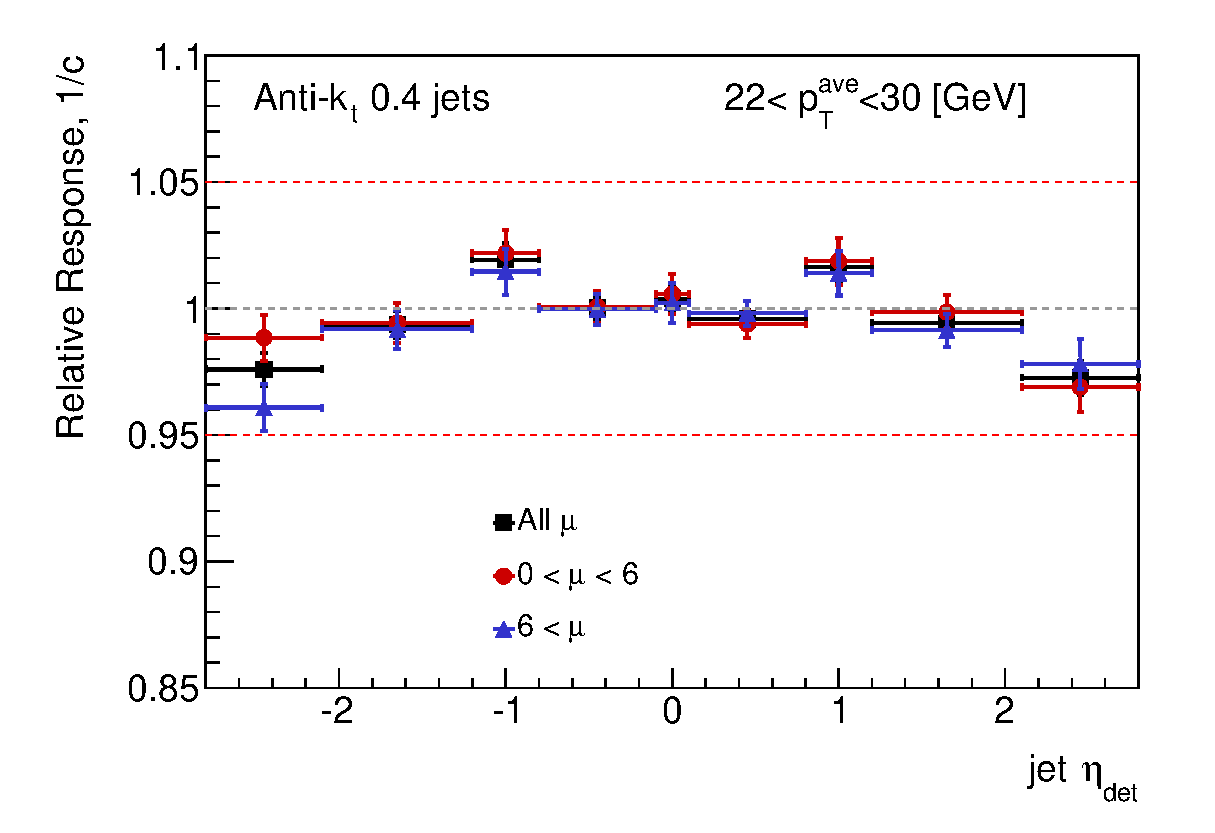
\includegraphics[width=0.9\textwidth]{figures/JetPerformance/2011/Responsemuj10Comp.eps}
\caption[Relative response as a function of $\eta$ for 2 different pile-up conditions, based on $\mu{}$, for jets with $22<\ptave{}<30$ GeV]{
Relative response as a function of detector $\eta$ for jets with $22<\ptave{}<30$ GeV.
Relative responses are shown for events with \Range{\mu}{0}{6}, $\rm \mu\ge6$ and all $\mu$. 
\label{JetPerf:MuComp_j10}}
\end{figure}



\begin{figure}
\centering
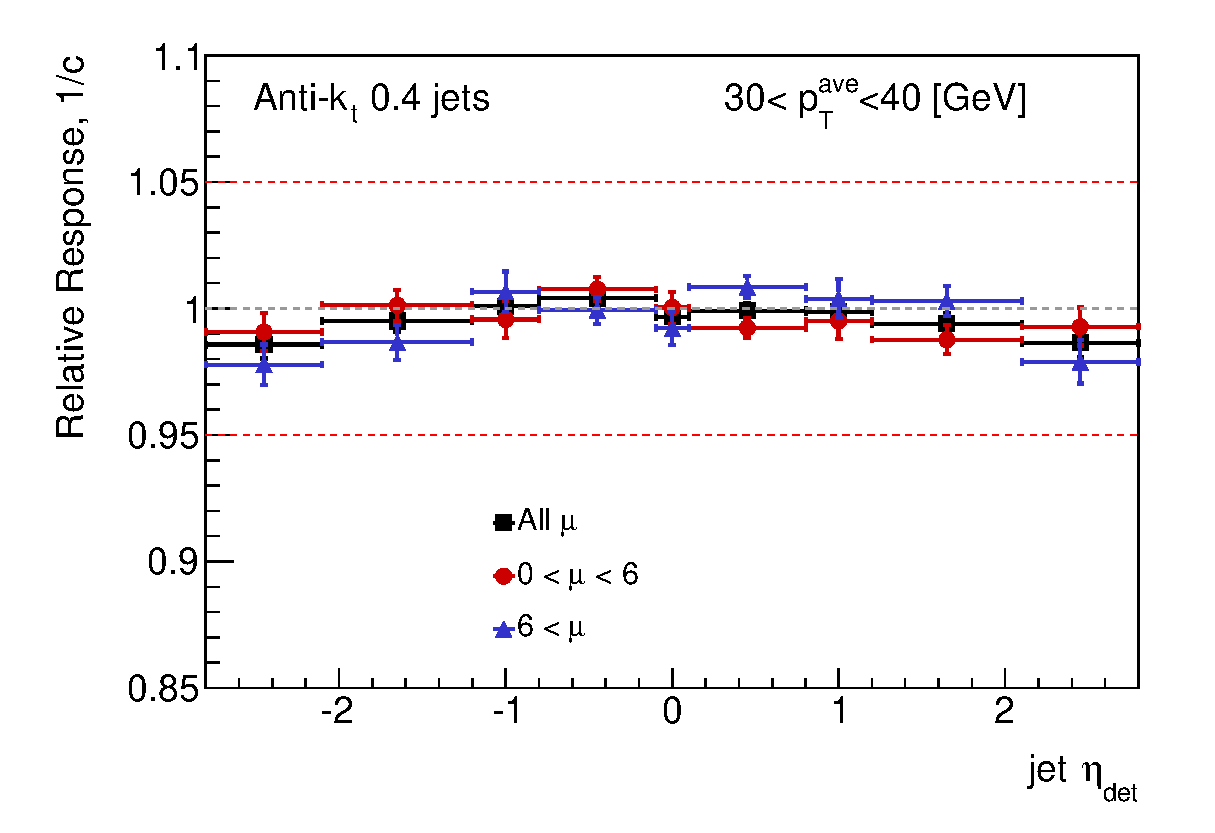
\includegraphics[width=0.9\textwidth]{figures/JetPerformance/2011/Responsemuj15Comp.eps}
\caption[Relative response as a function of $\eta$ for 2 different pile-up conditions, based on $\mu{}$, for jets with $30<\ptave{}<40$ GeV]{
Relative response as a function of detector $\eta$ for jets with $30<\ptave{}<40$ GeV.
Relative responses are shown for events with \Range{\mu}{0}{6}, $\rm \mu\ge6$ and all $\mu$. 
\label{JetPerf:MuComp_j15}}
\end{figure}

\begin{figure}
\centering
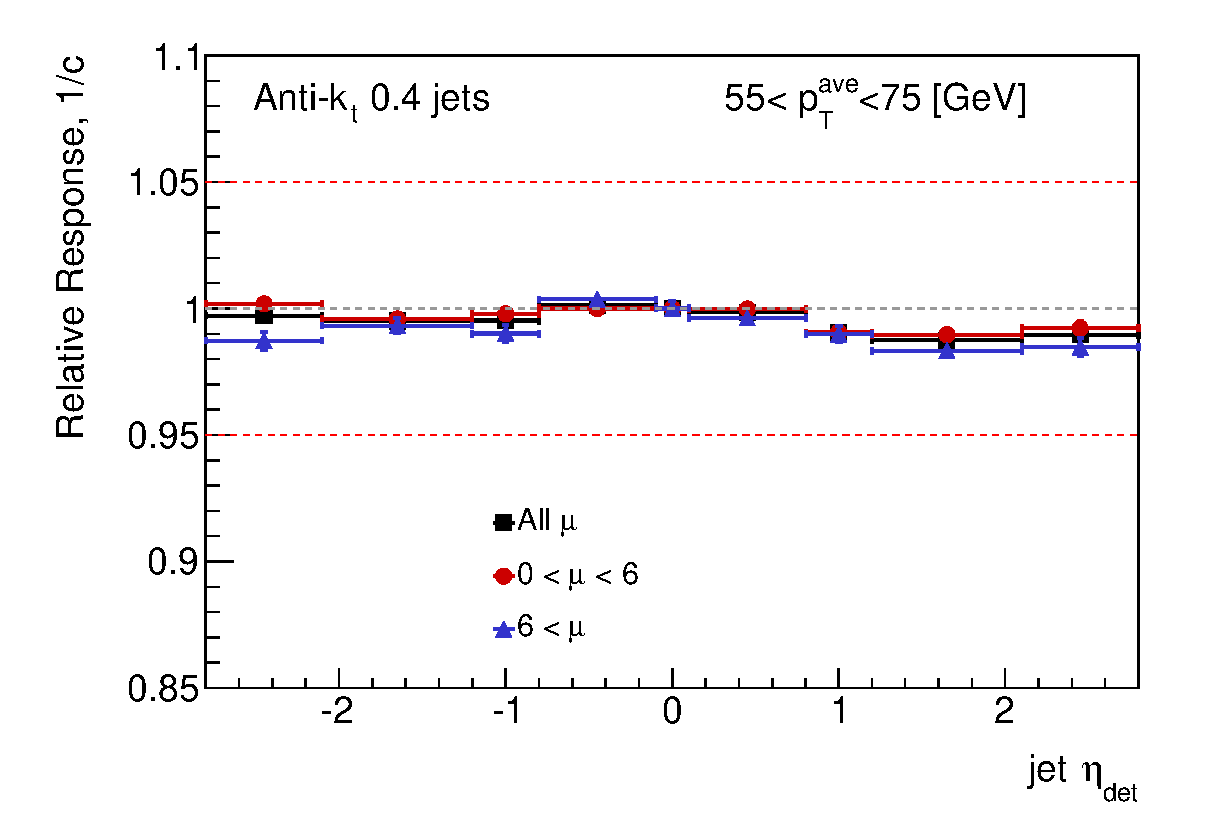
\includegraphics[width=0.9\textwidth]{figures/JetPerformance/2011/Responsemuj30Comp.eps}
\caption[Relative response as a function of $\eta$ for 2 different pile-up conditions, based on $\mu{}$, for jets with $55<\ptave{}<75$ GeV]{
Relative response as a function of detector $\eta$ for jets with $55<\ptave{}<75$ GeV.
Relative responses are shown for events with \Range{\mu}{0}{6}, $\rm \mu\ge6$ and all $\mu$. 
\label{JetPerf:MuComp_j20}}
\end{figure}

